\documentclass[12pt, fullpage]{article}
\usepackage{amssymb,latexsym,amsmath,amscd,epsfig,amsthm,graphicx}

\newcommand*{\QEDA}{\hfill\ensuremath{\blacksquare}}%
\pagestyle{empty}

\input epsf
\newdimen\epsfxsize

\parindent=0pt
%\setlength{\evensidemargin}{-2.0cm}
%\setlength{\oddsidemargin}{-1.0cm}
\setlength{\topmargin}{-2.2cm}
%\setlength{\baselineskip}{20pt}
%\setlength{\textwidth}{19cm}
%\setlength{\textheight}{23cm}

\newcommand{\ds}{\displaystyle}
\newcommand{\un}{\underline}
\newcommand{\R}{\mathbb R}
\newcommand{\Z}{\mathbb Z}


\begin{document}
\begin{flushleft}
\textbf{Nilay Bhatt Feb. 8 2017}		
\end{flushleft}
\begin{center}
	\textbf{Results about Euler's path and circuits}
\end{center}
\begin{center}
		
{\bf MATH 450 Seminar in Proof}
 \\
\end{center}
\textbf{Definition 1.1: \textit{Graph: }}A \textbf{graph} $G$ consists of a non-empty finite set $V(G)$ of elements called \textbf{vertices},
and a finite family $E(G)$ of unordered pairs of (not necessarily distinct) elements
of $V(G)$ called \textbf{edges}; the use of the word 'family' permits the existence of multiple edges. We call $V(G)$ the vertex set and $E(G)$ the edge family of $G$. An edge $e_{vw}$ is said to join the vertices $v$ and $w$, and is usually abbreviated to $vw$. \\

\textbf{Note:}	The vertices in $G$ are referred to as $V(G)$ and the edges on $G$ are referred to $E(G)$. This is independent of the way we define a graph. Meaning, if we define a graph $H = (W,Q)$ the set of vertices in $H$ is referred as $V(H) = W$ and the set of edges in $H$ is referred as $E(H) = Q$ and not $W(H)$ and  $Q(H)$ respectively.\\

\textbf{Definition 1.2: \textit{Adjacency:}}: We say that two vertices $v$ and $w$ of a graph $G$ are \textbf{adjacent} if there is an edge $vw$ joining
them, and the vertices $v$ and $w$ are then \textbf{incident} with such an edge. Similarly, two
distinct edges $e$ and $f$ are \textbf{adjacent} if they have a vertex in common.\\

\textbf{Definition 1.3: \textit{Degree of a Vertex:}}: The degree of a vertex $v$ of $G$ is the number of edges connected with $v$, and is written
$deg(v)$; in calculating the degree of $v$, we usually make the convention that a loop at $v$
contributes 2 (rather than 1) to the degree of $v$. A vertex of degree 0 is an \textbf{isolated} vertex and a vertex of degree 1 is an \textbf{end-vertex}.\\

\textbf{Note:} A graph is \textit{\textbf{connected}} if it cannot be expressed as the union of two distinct graphs, and \textbf{disconnected} otherwise. \\

\textbf{Definition 1.4: \textit{Subgraph:}}:A \textbf{subgraph} $H$ of a graph $G$ is a graph, such that $V(H) \subseteq V(G)$ and $E(H) \subseteq E(G)$.\\

\textbf{Definition 1.5: \textit{Walk}}: Given a graph $G$, a \textbf{walk} in $G$ is a finite sequence of distinct edges of the form $v_0v_1$, $v_1v_2$,...,$v_{m-1}v_m$, also denoted by $v_0 \rightarrow v_1 \rightarrow v_2 \rightarrow ....\rightarrow v_m$, in which any two consecutive edges are adjacent.  If $v_0 = v_m$ then we call the walk a \textbf{cycle}.\\

\textbf{Definition 1.6: \textit{Euler Path: }}An \textbf{Euler Path} on a graph $G$ is a special walk that uses each edge exactly once.\\

\textbf{Definition 1.7: \textit{(Euler Circuit/Cycle: }}An \textbf{Euler circuit} on a graph $G$ is an Euler Path with a cycle.\\

\textbf{Definition 1.8: \textit{Traversing: }}The process of passing through each vertex of a  walk or cycle in a graph $G$ using the edges joining them in a walk or a path or a cycle.\\ \\

\textbf{Lemma: \textit{Nilay's Lemma (Not really):}} If a connected graph has every vertex of degree of at least two, then $G$ has a \textit{cycle}.
\begin{proof}
Let $G$ be a connected graph. Let $v$ be a vertex in $G$ such that $v$ has at least degree two. Let us construct a walk $v_0 \rightarrow v_1 \rightarrow v_2 \rightarrow ....$ such that $v_1$ be any adjacent vertex to $v_0$, and for each $v_i$ $i > 1$, we choose $v_{i+1}$ to be any adjacent vertex to $v_i$, except $v_{i-1}$(already chosen). We know that such a vertex exists because of our hypothesis that every vertex is of at least degree two. Since $G$ is finite graph, the number of vertices it has is finite. Thus, while constructing our walk we will eventually choose a vertex $v_k$ which has already been chosen and included in the walk. If $v_k$ is first such vertex that we encounter,then the path that was created from the first occurrence of $v_k$ to the second one is a cycle from $v_k$ to $v_k$.
\end{proof}



\textbf{\\Results to be proven: }

\begin{enumerate}
	\item \textit{\textbf{(EULER (1736), HIERHOLZER (1873))}} A connected graph $G$ has an Euler Circuit if and only if the degree of each vertex of $G$ is even.
\begin{proof}
 	$\Longrightarrow$ Let $G$ be a connected graph which has Euler circuit $C$. Whenever $C$ passes through a vertex in $V(G)$ through an edge in $E(G)$,there is a contribution of 2 edges which are adjacent to the vertex, towards the degree of that vertex. Since each edge occurs exactly once in $C$, each vertex must have even degree. \\
 	
 	$\Longleftarrow$ Let us proceed by induction. . In a most basic connected graph $G$ of no edges and one vertex, the proposition is vacuously true. If a connected graph $G$ has one vertex $v \in V(G)$, then the number of edges in $E(G) = 1$, thus we start and end our Euler Circuit at $v$ (loop, contribution of 2 towards the degree). \\
 	
 	Now, let there be only two vertices in a connected graph $G$ and each vertex is of degree two (making them even degree). Then since $G$ is connected, there are no isolated vertex in $G$. Furthermore, those two vertices share the two edges between them. Therefore, if we construct a walk at either of the vertex in $V(G)$ we will end at the same vertex where we started, and not repeating the edge that we passed through. Thus making the walk a Euler Circuit.\\ 
 	
 	Now by our strong induction hypothesis, we say, if $G$ is a graph, $\forall v \in V(G)$ having an even degree and where $\vert E(G)\vert \leq k, k \in \Z$, there is an Euler Circuit in $G$.\\
 	
 	 Now, let $G$ be connected graph with $k+1$ vertices, where each vertex in $G$ is of even degree. From the lemma we know that there exists a cycle in $G$. If a cycle includes all the edges in $G$ then we are done. Let's say it does not. Then there exists a cycle $C$ in $G$ which does not include all the vertices of $G$ . 
 	 
 	 Now, let us remove all the edges from $G$ that are in $C$ and obtain newly made sub-graph $H = (V(G) - V(C) , E(G)-E(C))$, made by the remaining edges in $G$, by our hypothesis all the vertices in $H$ are still even. We know this because when we removed $E(C)$ from $E(G)$, we removed an even number of edges from the cycle $C$ formed in $G$.\\
 	 
 	  If $H$ is still connected, $i.e.$ there are no isolated vetices in $H$ then we get a graph with less than $k$ edges, and thus $H$ has a Euler Circuit from our hypothesis because $\vert E(H) \vert < k$. Furthermore, since $H$ is connected, there must be a common vertex $m \in V(C) \cap V(H)$. So, now we have a Euler circuit in $G$, where we start from any vertex $v \in V(C)$ and while traversing $C$, when we reach $m$, we traverse the Euler Circuit in $H$, starting and ending at $m \in V(C) \cap V(H)$ and ending our cycle at $v$, thus traversing along all the edges in $E(G) = E(C) \cup E(H)$ once and all the vertex in $V(G) = V(C) \cup V(H)$.
 	 
 	   When we removed $C$ from $G$, the other possibility was that we may have $H$ disconnected. Thus $H = H'_1 \cup H'_2 \cup H'_3 ... \cup H'_i$. $H$ is formed from a disjoint union of such even degree connected sub-graph $H_i$. Note that, for each such $H_i$, $\exists v_i \in V(C) \cap V(H_i)$. Since $\forall i, \vert E(H'_i) \vert < k$, from our hypothesis, each such $H_i$ has a Euler Circuit, made by one $C'_i$, or multiple cycles $C_{i_j}$.
 	   
 	   We can now build an Euler circuit for $G$. Pick an arbitrary vertex $a \in V(C) \subset V(G)$ from $C$. Traverse along $C$ starting from $a$ until we reach a vertex $v = V(C) \cap V(H')$. Then, traverse along its Euler circuit starting from $v$ made by the cycle $C'$ in $H'$. 
 	   
 	   Now we are back to $v$, and so we continue along $C$, and do the same for each such $v_i \in V(C) \cap V(H'_i)$ we encounter and after traversing each edge in $E(G) = E(C) \cup E(H'_1)\cup E(H'_2) \cup E(H'_3)... \cup E(H'_i)$ exactly once and all the vertices in $V(G) = V(C) \cup V(H'_1)\cup V(H'_2) \cup V(H'_3)... \cup V(H'_i)$, we get our desired Euler path in $G$ starting and ending at $a \in V(G)$.
 	  %Now since $v$ still has an even degree we produce a cycle $C'$ in $H$ that starts and ends at $v$. Now the cycle formed by combining $C'$ in $H$ and $C$ in $G$ forms a new cycle in $G$, that starts and ends at $v$ and containing more edges than in $C$.\\
 	  %We continue the above process recursively for each sub-graph in $G$ until all the vertices in $G$ are traversed. The final cycle starting from such a vertex $v$ will include all the edges in $G$ and will be the union of all the cycles that we created recursively in $G$ and it's sub-graphs, thus making an Euler circuit in $G$.\\
 	  
 	  They say a picture speaks a thousand words, below we try to illustrate what an Euler Circuit will look like on a graph where all the vertex have an even degree.
\end{proof} 
\begin{figure}[h!]
  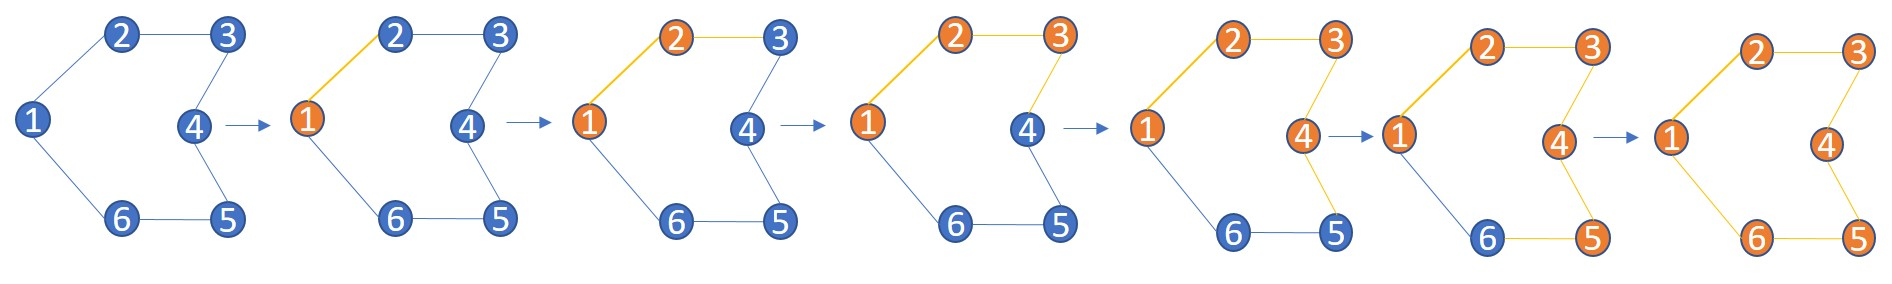
\includegraphics[width=\linewidth]{circuit.jpg}
  \caption{A Euler Circuit.}
\end{figure}
\newpage
\item If there are exactly two vertices $a$ and $b$ of odd degree, there is an Euler path on the graph from $a$ to $b$. (Existence Proof)
\end{enumerate}
\begin{proof}	
	Let $G$ be a graph with Euler circuit. Thus, we know that every vertex in $G$ has an even degree from the theorem stated above. Now let us add one vertex say $b \notin V(G) $ and an edge $e_{ba} \notin E(G)$ to a vertex $a \in V(G)$. Note that before adding the edge  from $e_{ba}$ to $a$, $a \in V(G)$ had an even degree. We start our path from $b$, and since it has only one edge $e_{ba}$ connecting to $a$. We know that $a \in V(G)$ and since $G$ has a Euler Circuit, we know that we can construct a cycle that starts and ends at $a \in G$. We cannot use the edge $e_{ba}$ to go back to $b$ as we have already included in our path. Therefore, the path will end at $a$. Thus, we know have a graph $G' = (V(G) + b, E(G) + e_{ba})$, where $a$ and $b$ are two vertices in $G'$ that are of odd degree and an Euler Path starting from $b$ and ending at $a$.

\end{proof}

\end{document}